\documentclass{article}
\usepackage[utf8]{inputenc}
\usepackage{caption}
\usepackage{color}
\usepackage{float}
\usepackage{graphicx}
\usepackage{parskip}
\usepackage{polski}
\usepackage[dvipsnames]{xcolor}
\usepackage{csquotes}
\usepackage{listings}

\graphicspath{ {images/} }

% Odległości między paragrafami oraz wcięcia
\setlength{\parskip}{1em}
\setlength{\parindent}{3em}

% Środowisko bez page-breaków, z zachowanymi odległościami między paragrafami oraz wcięciami
% NOTE: Póki co nie używane w treści licencjatu
\newlength{\currentparskip}
\newlength{\currentparindent}
\newenvironment{nopgbreak}
  {\setlength{\currentparskip}{\parskip}
   \setlength{\currentparindent}{\parindent}
   \begin{minipage}{\textwidth}
   \setlength{\parskip}{\currentparskip}
   \setlength{\parindent}{\currentparindent}
  }
  {\end{minipage}}

% Grafiki bez wcięć akapitu
\let\oldincludegraphics\includegraphics
\renewcommand{\includegraphics}[2][]{\noindent\oldincludegraphics[#1]{#2}}

% Specjalne oznaczenia
\newcommand{\name}[1]{\textbf{\textcolor{NavyBlue}{#1}}}
\newcommand{\todoadrian}{\textbf{\textcolor{red}{<< TO MIEJSCE WYPEŁNIA ADRIAN >>}}}
\newcommand{\todomateusz}{\textbf{\textcolor{red}{<< TO MIEJSCE WYPEŁNIA MATEUSZ >>}}}

% Podświetlanie składni C#
\definecolor{bluekeywords}{rgb}{0.13,0.13,1}
\definecolor{greencomments}{rgb}{0,0.5,0}
\definecolor{redstrings}{rgb}{0.9,0,0}
\lstset{language=[Sharp]C,
captionpos=b,
%numbers=left, %Nummerierung
%numberstyle=\tiny, % kleine Zeilennummern
frame=lines, % Oberhalb und unterhalb des Listings ist eine Linie
showspaces=false,
showtabs=false,
breaklines=true,
showstringspaces=false,
breakatwhitespace=true,
escapeinside={(*@}{@*)},
commentstyle=\color{greencomments},
morekeywords={partial, var, value, get, set},
keywordstyle=\color{bluekeywords},
stringstyle=\color{redstrings},
basicstyle=\ttfamily\small,
}

% Dane licencjatu
\title{Sieciowa fabularna\\gra komputerowa - The Trinity}
\author{Kleina Mateusz, Podlawski Adrian}
\date{12 kwietnia 2017}

\begin{document}

% Strona tytułowa
\begin{titlepage}
\maketitle
\tableofcontents
\end{titlepage}

\section{Wstęp i opis}
\subsection{Porównanie dostępnych rozwiązań}

\section{Projektowanie oraz przygotowanie środowiska}
\subsection{Projekt Terenu}
\subsection{Projekt Postaci sterowanych przez gracza}
\subsection{Projekt systemu mulitplayer}
\subsection{Instalacja niezbędnych narzędzi}

\section{Implementacja}
  \section{Budowa terenu}\label{sec:budowa_terenu}
Budowa podstawowej mapy gry jest stosunkowo nieskomplikowanym procesem, dzięki czemu mogliśmy się tutaj skupić głównie na projektowaniu dróg, rozłożeniu obiektów i kształtowaniu mapy na potrzeby rozgrywki.

\subsection{Przygotowanie terenu}

    Do przygotowania terenu został użyty specjalnie do tego przeznaczony typ obiektu 3D o nazwie \name{Terrain}. Po utworzeniu takiego obiektu w hierarchii obiektów na ekranie ukaże się nieoteksturowana płaszczyzna.

    \begin{figure}[H]
    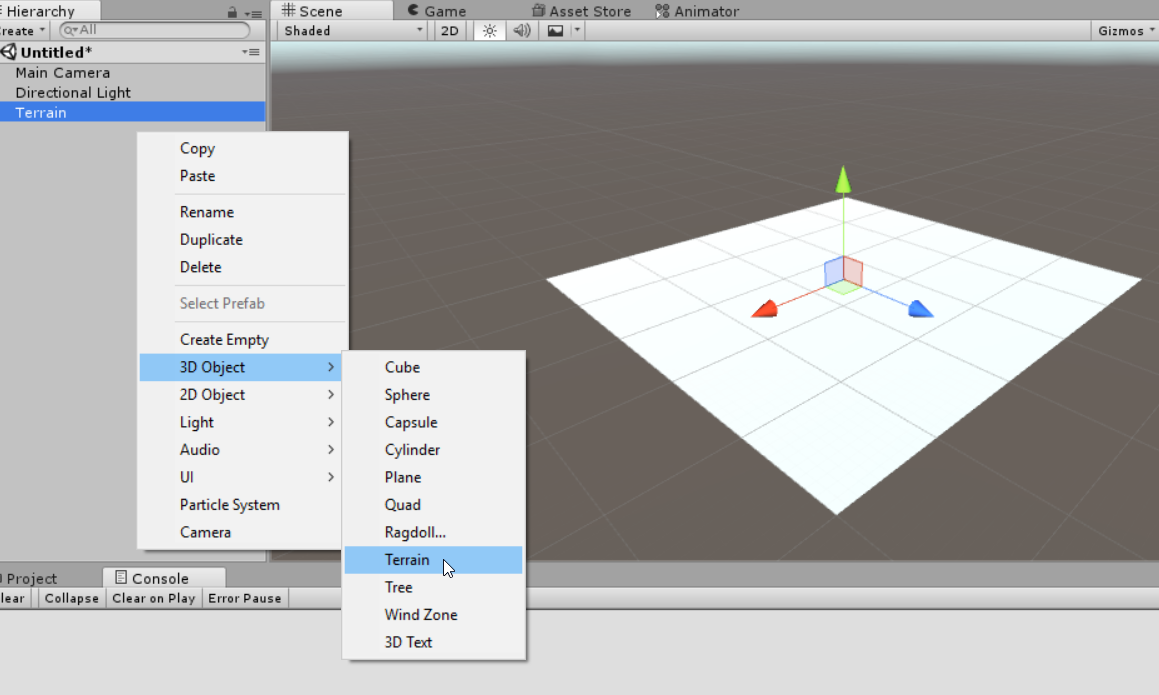
\includegraphics[width=\textwidth]{teren_1.png}
    \caption{Płaszczyzna terenu}
    \end{figure}

\subsection{Formowanie kształtu} 

    Na tak przygotowanej płaszczyźnie uformowane zostały nierówności przy użyciu palety narzędzi terenu. Używając opcji \name{Raise / Lower Terrain} utworzone zostały wypiętrzenia nadające kształt mapie gry. Charakter wypiętrzeń dostosowany został używając odpowiedniego pędzla z panelu \name{Brushes}, natomiast promień zniekształceń oraz siła efektu za pomocą parametrów kolejno \name{Brush Size} oraz \name {Opacity}.

    \begin{figure}[H]
    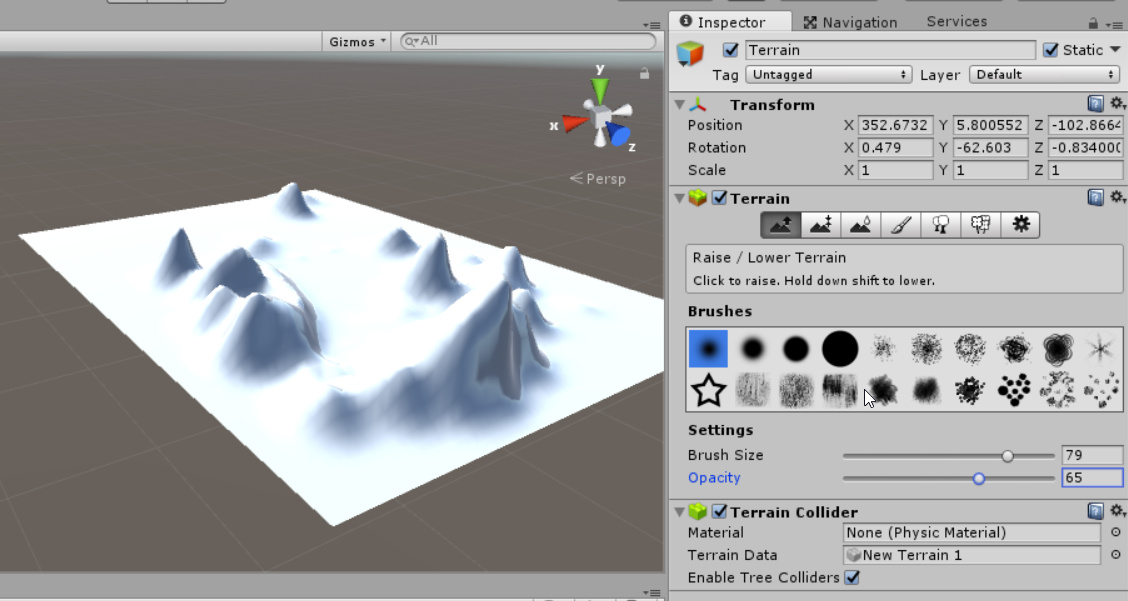
\includegraphics[width=\textwidth]{teren_2.png}
    \caption{Modelowanie nierówności terenu}
    \end{figure}

\subsection{Nakładanie tekstur}

    Kolejnym krokiem było utworzenie tekstury służącej do nadaniu naszemu terenowi koloru oraz faktury. Do tego celu pobrane zostały odpowiednie tekstury z wbudowanego sklepu assetów \name{Asset Store}. Assety są rodzajem pakietów zawierających różnorakie obiekty, skrypty oraz tekstury, dostępne do pobrania z serwerów Unity.

    Po pobraniu odpowiedniej tekstury trawy, zostaje ona zaimportowana do folderu \name{Assets} znajdującego się w głównym katalogu projektu.

    Po wybraniu narzędzia \name{Paint Texture} ukazuje się panel \name{Textures} pozwalający na skonfigurowanie używanej przez narzędzie tekstury. Znajduje się tam przycisk \name{Edit Textures...} po kliknięciu którego otwiera się okno konfiguracyjne tekstury pozwalające na wybór tekstury podstawowej oraz tekstury przechowującej dane o chropowatościach. Po skonfigurowaniu tekstur i nałożeniu ich na teren, całość prezentuje się następująco.

    \begin{figure}[H]
    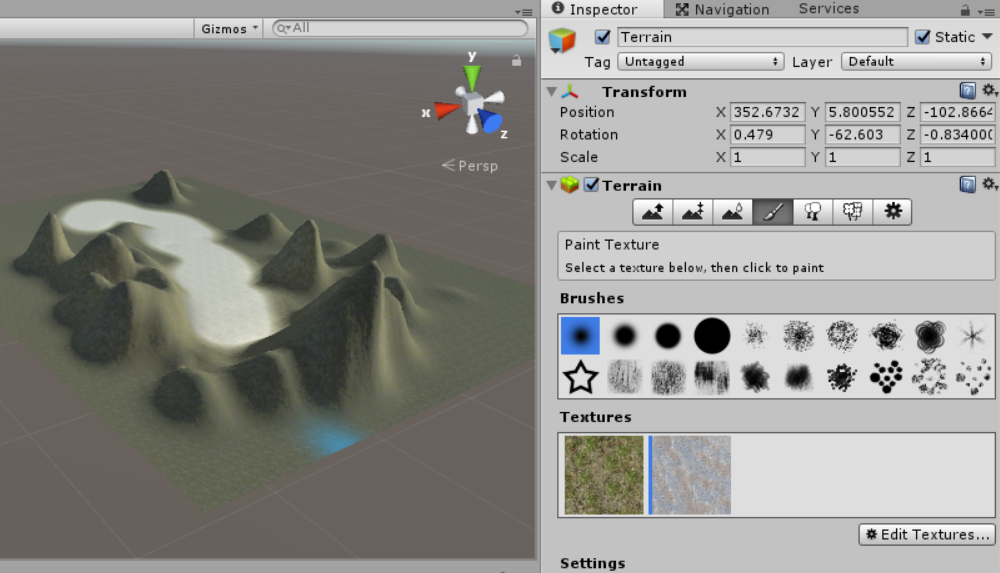
\includegraphics[width=\textwidth]{teren_3.png}
    \caption{Nakładanie tekstur na mapę terenu}
    \end{figure}

\subsection{Rozmieszczanie obiektów}

    Kolejnym krokiem w tworzeniu świata gry było umieszczenie na mapie sprefabrykowanych wcześniej obiektów (tzw. \textit{Prefabs}, o tym później). Wszystkie obiekty użyte w pracy są dostępne za darmo w bibliotece obiektów Unity (\name{Asset Store}). Po pobraniu, obiekty znajdują się w podfolderze \name{Prefabs} zainstalowanej paczki. Obiekty umieszcza się na mapie metodą przeciągnij-upuść, dostosowując ich koordynaty używając narzędzi transformacji dostępnych w pasku narzędzi znajdującym się w górnej części okna edytora.

    \begin{figure}[H]
    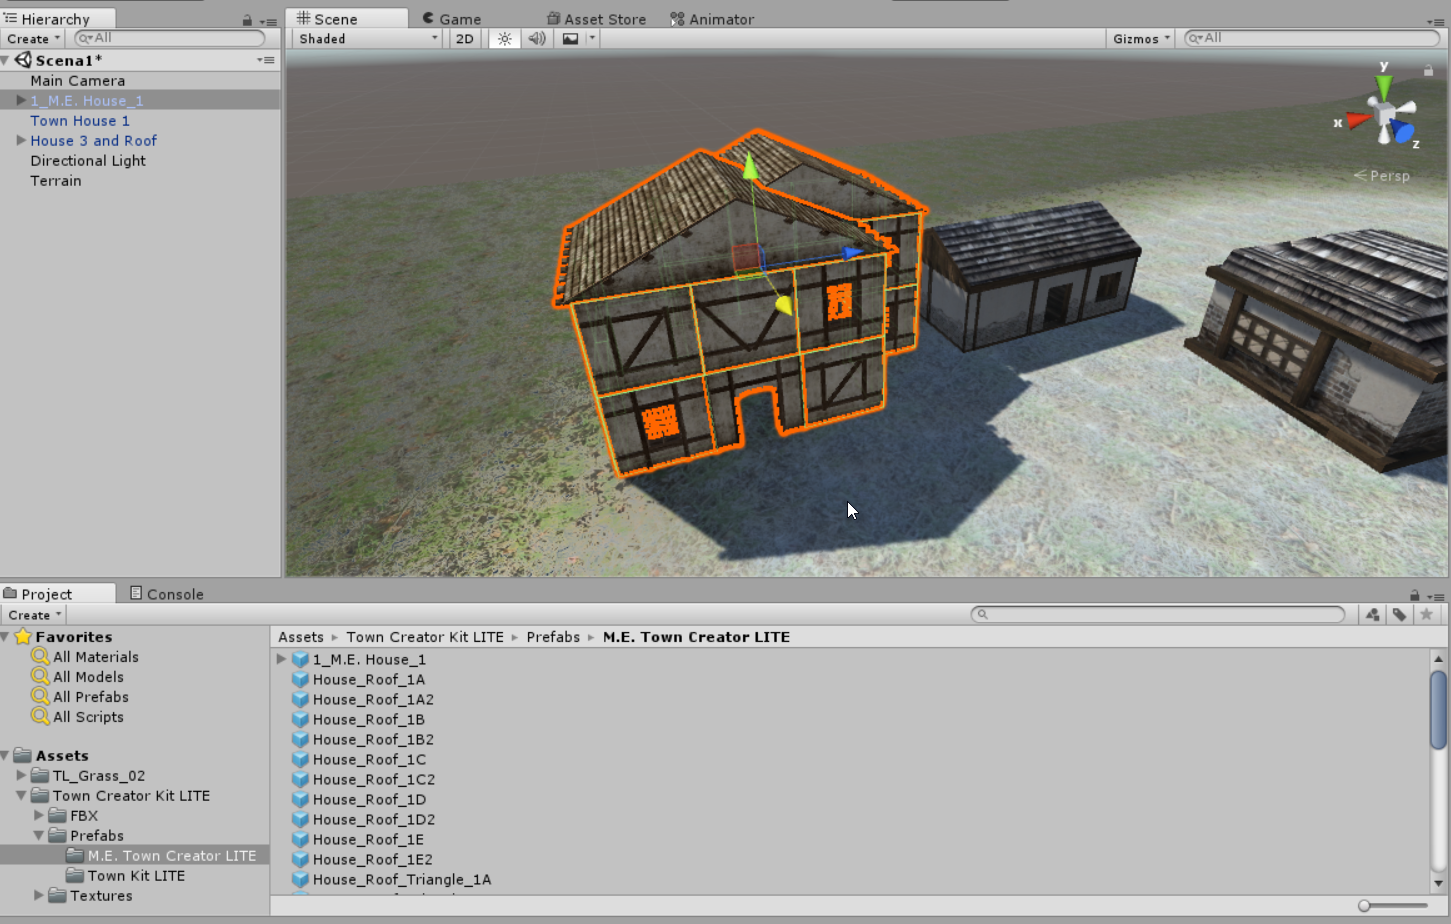
\includegraphics[width=\textwidth]{teren_obiekty.png}
    \caption{Umieszczanie obiektów na mapie}
    \end{figure}

    % Szczegóły kolizji w sekcji~\ref{sec:fizyka} na stronie~\pageref{sec:fizyka}

\subsection{Oddziaływanie terenu na inne obiekty}

    Kluczowym elementem tworzenia mapy świata gry są takie elementy jak oddziaływanie na postacie ograniczeń nachylenia terenu typu wzgórza, drzewa, czy budynki, uniemożliwiających dostanie się w niektóre miejsca. Unity w celu uproszczenia obliczeń posiada możliwość wygenerowania uproszczonej mapy dróg (tzw. \textit{NavMesh}) na bazie modelu terenu, pozwalającej na dynamiczne omijanie przeszkód przez wroga (o tym później w sekcji \ref{sec:poruszanie_wrogow} na stronie \pageref{sec:poruszanie_wrogow}).

    Aby utworzyć taką mapę, należy przejść do zakładki \name{Navigation}, gdzie w panelu \name{Bake} znajduje się lista parametrów dotyczących maksymalnego kąta nachylenia terenu, czy maksymalnej wysokości uskoku, którą obiekty sterowane przez komputer mogą pokonać.

    \begin{figure}[H]
    \center
    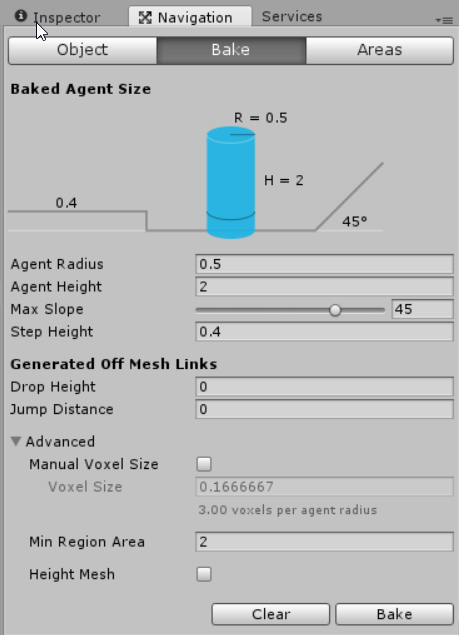
\includegraphics[width=6cm]{teren_obiekty2.png}
    \caption{Parametry mapy dróg}
    \end{figure}

    Po ustaleniu parametrów i kliknięciu przycisku \name{Bake}, mapa zostaje wygenerowana, natomiast w oknie widoku sceny, obszary dostępne do przemierzania oznaczone zostają niebieskim kolorem. Operację można powtarzać do uzyskania optymalnych efektów.

    \begin{figure}[H]
    \center
    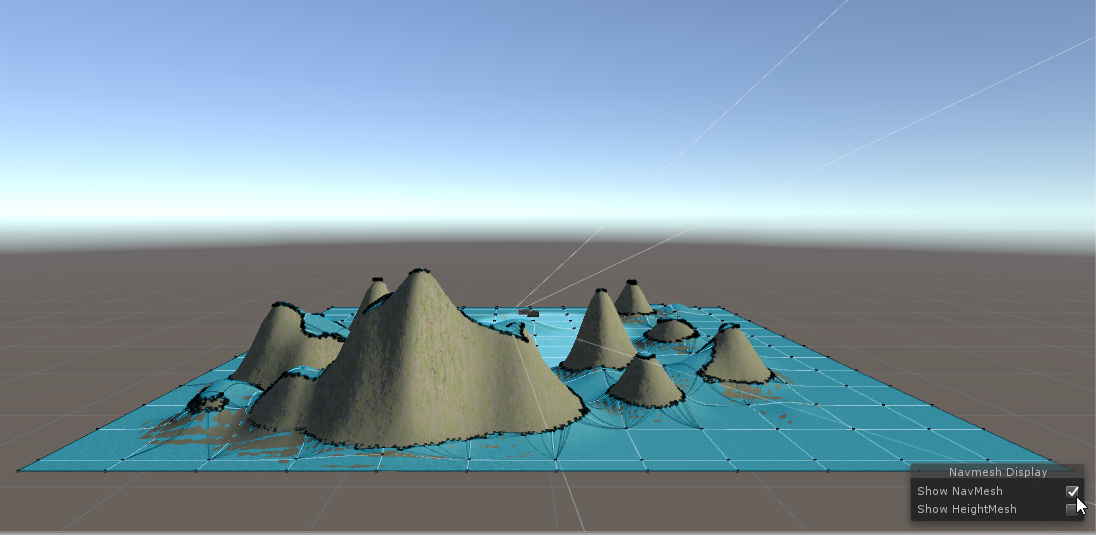
\includegraphics[width=9cm]{teren_obiekty3.png}
    \caption{Poprawnie wygenerowany \textit{NavMesh}}
    \end{figure}

    Tak przygotowana mapa posłużyła nam do projektowania dalszej części gry.

    % Każdy obiekt utworzony w Unity posiada paletę komponentów. Komponenty pozwalają na określanie właściwości obiektów, takich jak rozmiar, pozycja, czy masa. Komponentami są również skrypty, pozwalające na określenie interacji obiektu z zewnętrznym światem (np. zdarzenie \textit{OnCollisionEnter}).
  \subsection{Tworzenie Postaci}
  \todoadrian
  \subsection{Ruch kamery}

\paragraph{Pozycja kamery}

    Widok w grze jest trzecioosobowy, kamera obejmuje zarówno widzialny obszar jak i samego gracza. Pod tym względem jest to gra TPP (\textit{Third Person Perspective}). Przykładowymi grami tego typu są bardzo znane produkcje, takie jak seria \textit{Wiedźmin}, \textit{Tomb Raider}, czy \textit{GTA}.

    Aby uzyskać efekt kamery podążającej za graczem, obiekt kamery powinien zostać umieszczony wewnątrz obiektu gracza w hierarchii obiektów. W ten sposób koordynacje kamery będą ustawiane względem gracza, a sama kamera poruszać się będzie i obracać wraz z nadrzędnym obiektem.

    Koordynacje kamery ustawiliśmy na (0, 0, 0), w ten sposób kamera jest w środkowym punkcie obiektu nadrzędnego i wytarczy za pomocą narzędzi transformacji przesunąć ją do oczekiwanej pozycji (tak, aby obejmowała obraz zza pleców postaci). Inną, bardziej poręczną metodą jest odpowiednie dostosowanie widoku sceny i skopiowanie jego koordynatów do zaznaczonej w hierarchii kamery.

    \begin{figure}[H]
    \center
    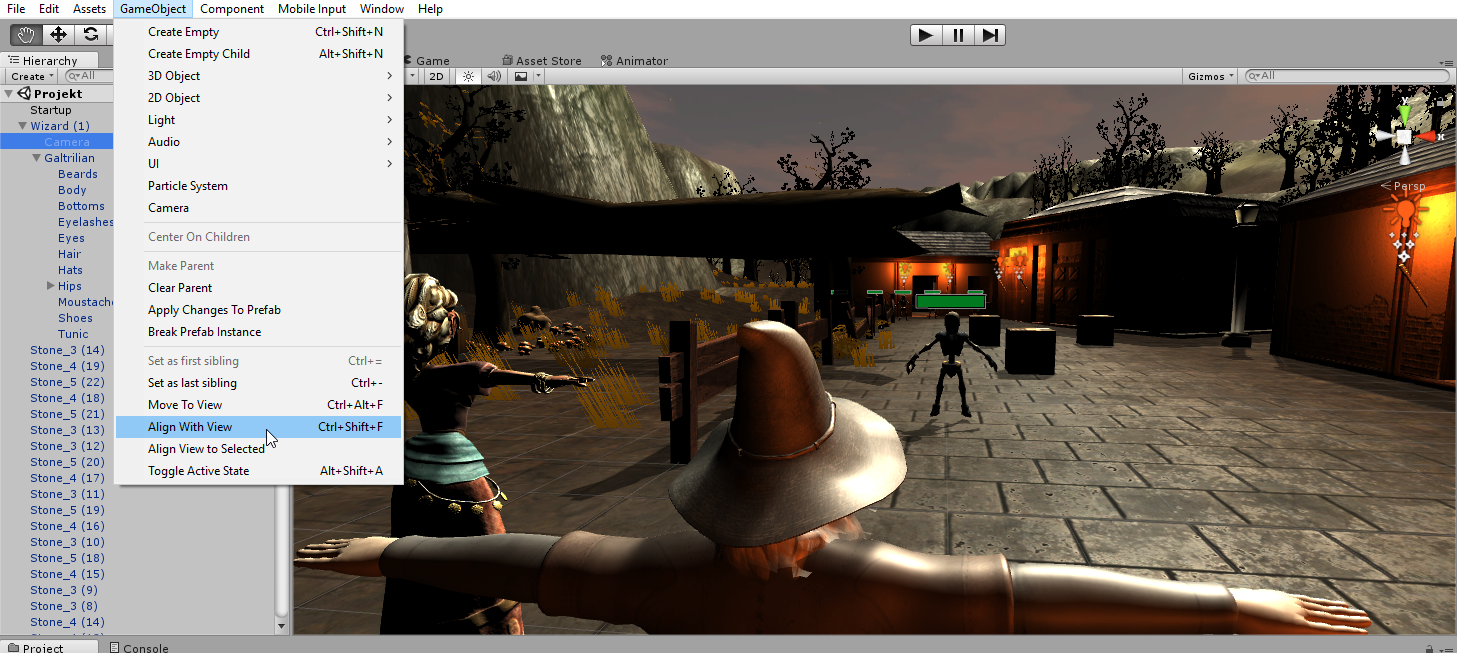
\includegraphics[width=\textwidth]{kamera_1.png}
    \caption{Dostosowanie pozycji kamery gracza względem aktualnego widoku sceny}
    \end{figure}

\paragraph{Mechanika obrotu kamery}

Kolejnym etapem jest oprogramowanie ruchu kamery za pomocą ruchów myszy. Mysz jest używana również do obrotu postacią. Jako, że kamera \enquote{przyklejona} jest do postaci, aby uzyskać efekt rozglądania się, modyfikujemy jedynie jej obrót w pionie, natomiast ruch myszy w poziomie obraca poziomo całą postać wraz z kamerą.

\begin{figure}[H]
\center
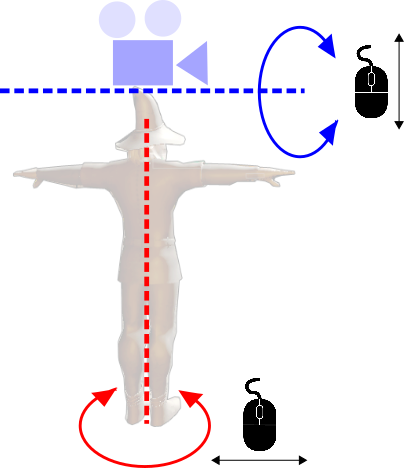
\includegraphics[width=9cm]{kamera_2.png}
\caption{Schemat działania systemu sterowania kamerą}
\end{figure}

\begin{lstlisting}[caption={Obrót kamery za pomocą myszy}]
if (!photonView.isMine) return;
if (!stopCamera)
{
    Camera.main.transform.Rotate(new Vector3(-Input.GetAxis("Mouse Y") * rotationSensitivity * Time.deltaTime, 0, 0));
    rb.transform.Rotate(new Vector3(0, Input.GetAxis("Mouse X") * rotationSensitivity * Time.deltaTime, 0));
}
\end{lstlisting}

Obrót kamery polega na dodaniu wektora obrotu do odpowiedniej osi kamery, natomiast wielkość wektora określona jest przez wartość chwilowego przesunięcia myszy, skalowanego parametrem \textit{rotationSensivity} w celu określenia czułości myszki. Parametr \textit{Time.deltaTime} zwraca czas od ostatniej wyrenderowanej klatki, co pozwala na uzyskanie jednolitej czułości myszki bez względu na ilość generowanych klatek na sekundę.

\paragraph{Celownik}

Aby ułatwić celowanie w przeciwników oraz interakcję z otoczeniem umieściliśmy w grze celownik, który w dalszym etapie tworzenia gry zmienia kolor informując o możliwej interakcji.

Celownik jest obiektem 2D nałożonym na ekran w formie \textit{Sprite'a}. Sprite'y to 2-wymiarowe, wcześniej przygotowane obiekty graficzne. W naszym wypadku posłużyliśmy się bezstratnym formatem PNG.

Do sceny został dodany obiekt, na który nałożyliśmy komponenty \name{Canvas} oraz \name{CanvasScaler}. Nakładają one na ekran dwuwymiarowe płótno oraz pozwalają na skalowane go względem podanej rozdzielczości referencyjnej. Wewnątrz takiego płótna można umieszczać obrazy, elementy interfejsu oraz różnego rodzaju wskaźniki (np. Pasek postępu życia bohatera).

\begin{figure}[H]
\center
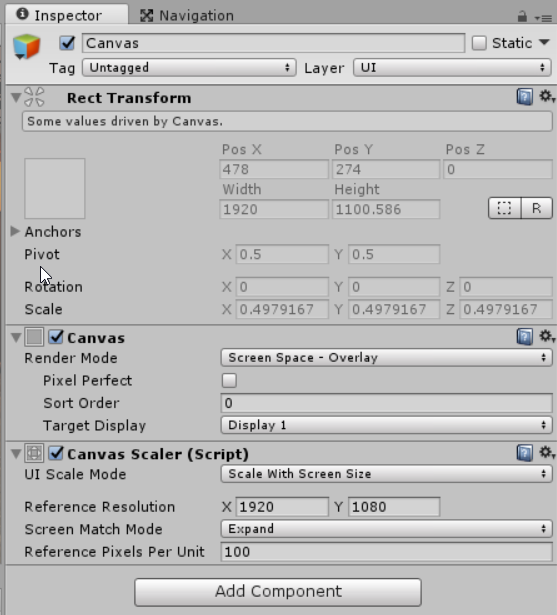
\includegraphics[width=5cm]{celownik_1.png}
\caption{Konfiguracja płutna 2D do wyświetlania interfejsu gry}
\end{figure}

Wewnątrz płótna został umieszczony obrazek (komponent \name{Image}) celownika, wyrównany do środka ekranu.

\begin{figure}[H]
\center
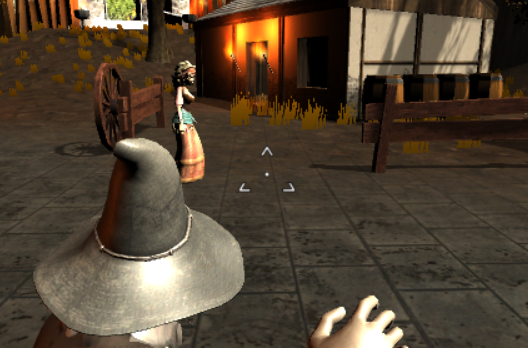
\includegraphics[width=6cm]{celownik_2.png}
\caption{Gotowy celownik gracza}
\end{figure}
  \section{Fizyka}\label{sec:fizyka}

Ważnym elementem gry jest fizyka, aby postaci mogły poruszać się, podskakiwać i reagować na kolizje.

Podstawowym komponentem zapewniającym obliczenia fizyczne jest \name{Rigidbody}. Komponent ten przyjmuje parametry takie jak wartość masy, tarcia, czy wyłączenie grawitacji.

Aby zdarzenia fizyczne mogły mieć miejsce, na elementy otoczenia oraz samą postać gracza nałożone powinny zostać komponenty \name{Collider}. Są to obszary określające granice kolizji. Mogą one mieć kształt kapsuły, sześcianu, bądź uproczczonego modelu samego obiektu. Pozwalają one silnikowi gry na przyspieszenie obliczeń i płynne reakcje na zdarzenia kolizji.

\begin{figure}[H]
\center
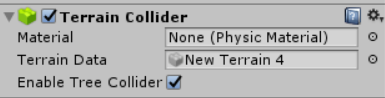
\includegraphics[width=6cm]{fizyka_1.png}
\caption{Przykład -- collider mapy terenu}
\end{figure}

W przypadku postaci poruszających się po mapie, zablokowane zostały obroty we wszystkich osiach (parametr \name{Freeze Rotation} komponentu Rigidbody), dzięki czemu nie przewracają się one na bok przy nierównościach terenu i kolizjach z otoczeniem. Zdarzenia fizyczne wyliczane są jedynie w pionie (spadanie, skok itp.).

\subsection{Mechanika skakania postaci}

Mając już zaimplementowaną fizykę, dodaliśmy możliwość skoku. Utworzona została metoda \textit{jump()}, która dodaje do zdarzeń fizycznych naszej postaci siłę w kierunku pionowym o wektorze ustalonym parametrem \textit{jumpPower}. Natomiast na podstawie kolizji z terenem ustalane jest, czy postać stoi na ziemi, dzięki czemu nie można wykonać kolejnego skoku będąc już w powietrzu.
\\
\begin{lstlisting}[caption={Fragment algorytmu skoku postaci}]
void Start()
{
    rb = GetComponent<Rigidbody>();
    anim = GetComponent<Animator>();
}

void jump()
{
    if (onGround)
    {
        onGround = false;
        rb.AddRelativeForce(new Vector3(0, jumpPower, 0));
        anim.SetTrigger("Jump");
    }
}

void OnTriggerEnter(Collider other)
{
    onGround = true;
}
\end{lstlisting}
  \subsection{Animacje}
  \todoadrian
  \section{Poruszanie bohaterów}

Poruszanie bohaterów działa na podobnej zasadzie jak mechanika skoku. Do zdarzeń fizycznych bohatera dodawana jest siła o wektorze skierowanym w kierunku określonym przez wciskany klawisz (W, S, A lub D).

W przypadku chodzenia, animacja zależna jest od kierunku, w którym porusza się postać (cofanie, chodzenie bokiem).

Dodatkowym elementem mechaniki poruszania jest bieg, który aktywowany jest poprzez wciśnięcie lewego klawisza Shift.

\begin{lstlisting}[caption={Fragment kodu mechaniki biegania -- reakcja na wciśnięcie klawisza \name{W}}]
run = Input.GetKey(KeyCode.LeftShift);
anim.SetBool("Sprint", run);
float speed = run ? runSpeed : walkSpeed;

...

if (Input.GetKey(KeyCode.W))
{
    rb.AddRelativeForce(Vector3.forward * speed, ForceMode.VelocityChange);
}
\end{lstlisting}
  \section{Poruszanie postaci wrogów}\label{sec:poruszanie_wrogow}

Poruszanie wrogów odbywa się autonomicznie. Droga jest wyliczana, a koordynacje postaci zmieniane są zgodnie z wyliczoną drogą, dzięki czemu postacie wroga przemieszczają się płynnie w kierunku zdefiniowanego celu.

Unity posiada mechanizm wyznaczania dróg na mapie terenu (więcej informacji na ten temat w dziale~\ref{sec:budowa_terenu} na stronie \pageref{sec:budowa_terenu}). Aby móc z niego skorzystać, dodaliśmy do postaci wroga agenta nawigacji \name{NavAgent}. Jest to komponent zajmujący się obliczeniami drogi i zarządzaniem przemieszczeniem i obrotem postaci w czasie. Podstawowym parametrem jest 3-wymiarowy wektór określający docelową pozycję, silnik gry zajmuje się wyliczeniem trasy prowadzącej do punktu.

Mechanika wrogów polega na wyszukiwaniu najbliżej znajdującej się postaci gracza, a następnie ustaleniu jej jako cel podążania wroga. W momencie, gry wróg znajduje się odpowiednio blisko, rozpoczyna atak.
\\
\begin{lstlisting}[caption={Algorytm zwracający wskaźnik do obiektu znajdującego się najbliżej, przy określonym maksymalnym promieniu poszukiwań}]
GameObject findNearestPlayer(float maxDistance)
{
    GameObject[] players = GameObject.FindGameObjectsWithTag("Player");
    GameObject nearestPlayer = null;
    float distance = maxDistance;
    foreach (GameObject player in players)
    {
        float distanceFromEnemy = Vector3.Distance(player.transform.position, transform.position);
        if (distanceFromEnemy < distance)
        {
            distance = distanceFromEnemy;
            nearestPlayer = player;
        }
    }
    return nearestPlayer;
}
\end{lstlisting}

\begin{figure}[H]
\center
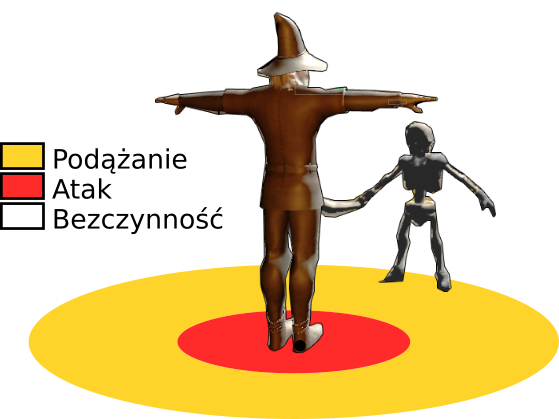
\includegraphics[width=\textwidth]{poruszanie_wrogow_1.png}
\caption{Obszary interakcji postaci wroga}
\end{figure}

W przypadku, gdy wróg ``widzi,, postać gracza, jest w jego stronę stale odwrócony. Służy do tego algorytm, który najpierw wylicza kierunek w postaci wektora wartości w skalu 0.0f..1.0f w przestrzeni 3D, a następnie zamienia wektor na kąt, do którego stopniowo dąży. Daje to efekt płynnego obracania postaci wroga z możliwością dostosowania prędkości obrotu, aby ruchy wyglądały naturalnie, a wróg dawał możliwość np. zajścia go od tyłu.
\\
\begin{lstlisting}[caption={Algorytm obracania postaci wroga w kierunku gracza}]
private void rotateTowards(Transform target)
{
    Vector3 direction = (target.position - transform.position).normalized;
    Quaternion lookRotation = Quaternion.LookRotation(direction);
    transform.rotation = Quaternion.Slerp(transform.rotation, lookRotation, Time.deltaTime * 5);
}
\end{lstlisting}

  \subsection{Nadanie bohaterom indywidualnych umiejętności}
  \subsection{Obrażenia}
  \subsection{Interakcja ze światem oraz NPC}
\end{document}
